\documentclass[
]{beamer}

\usepackage[english]{babel}
\usepackage[utf8]{inputenc}
\usepackage[T1]{fontenc}
\usepackage{lmodern}
\usepackage{csquotes}
\usepackage{expl3,biblatex}
\addbibresource{main.bib}
\usepackage{booktabs}
\usetheme[
  workplace=fi,
  fonts=none,
]{MU}
\usepackage{textalpha}
\usepackage{subfigure}
\usepackage{wrapfig}
\usepackage{tikz}
\usepackage{appendixnumberbeamer}

\title[Visualisation and Annotation of VolSeg Data in Mol*]{Lightweight Visualisation and Annotation of Volumetric and Segmentation Data in Mol*}
\subtitle[Master's Thesis Defense]{Master's Thesis Defense}
\author[D. Tichý]{Dominik Tichý\texorpdfstring{\\}{, }Advisor: RNDr. Tomáš Raček, Ph.D.}
\institute[FI MU]{Faculty of Informatics, Masaryk University}
\date{January 30, 2026}
\subject{Presentation Subject}
\keywords{Mol*, Mol* VS, MolViewSpec, MolViewStories, volumetric data, segmentations, visualization, bioinformatics}

\begin{document}

\begin{frame}[plain,noframenumbering]
\maketitle
\end{frame}

\begin{frame}{Motivation}
  \begin{itemize}
    \item Rapid growth of microscopy data (e.g., Cryo-EM, Cryo-ET) \cite{kuhlbrandt2014resolution}
    \item Critical in structural biology and drug design (e.g., SARS-CoV-2 spike protein characterization) \cite {wrapp2020covid}
    \item Need for a web-based tool to visualize and annotate
  \end{itemize}
\end{frame}

% TODO: add an image of the mol* vs architecture
\begin{frame}{Technologies}
  \begin{itemize}
    \item Mol* platform
    \item Mol* Volumes and Segmentation (Mol* VS)
    \begin{itemize}
      \item Difficult to use and maintain
      \item Lacks interoperability
      \item Siloed data formats
    \end{itemize}
    \item MolViewSpec (MVS)
    \begin{itemize}
      \item Declarative standard
      \item Describes ``what'' the scene looks like, not ``how'' to build it
    \end{itemize}
    \item MolViewStories
    \begin{itemize}
      \item UI builder for MolViewSpec
    \end{itemize}
  \end{itemize}
\end{frame}

\begin{frame}{Mol* VS Architecture}
  \begin{figure}
    \includegraphics[width=1\textwidth,height=0.8\textheight,keepaspectratio]{./images/volseg-arch.pdf}
    % \caption{Mol* VS Architecture}
  \end{figure}
\end{frame}


\begin{frame}{Goals}
  \begin{itemize}
    \item Move the legacy Mol* VS Client to MolViewSpec
    \item \textbf{Contribution 1:} Create a Python Conversion Library (CVSX → MVSX/MVStory)
    \item \textbf{Contribution 2:} Web application for non-technical users to convert, edit, and share biological stories
  \end{itemize}
\end{frame}

% TODO: add an image of a volume, it's segmentation, and annotation
\begin{frame}{Data Representation}
  \begin{itemize}
    \item \textbf{Volumes:} 3D scalar grids representing electron density or potential
    \item \textbf{Segmentations:} Convert intensity signals into discrete objects
    \begin{itemize}
      \item Lattice
      \item Meshes
      \item Geometric primitives
    \end{itemize}
    \item \textbf{Annotations:} Define semantic meaning and visual styling
  \end{itemize}
\end{frame}

\begin{frame}{Conversion Library --- Data Mapping}
  \begin{figure}
    \includegraphics[width=1\textwidth,height=1\textheight,keepaspectratio]{./images/mapping.pdf}
    \caption{Mapping CVSX to MVSX}
  \end{figure}
\end{frame}

\begin{frame}{Conversion Library --- Architecture}
  \textbf{``ETL'' Architecture:}
  \begin{itemize}
    \item \textbf{Extract:} Validate and parse CVSX
    \item \textbf{Transform:} Convert to intermediate representation
    \item \textbf{Load:} Serialize to MVSX or MVStory format
  \end{itemize}
\end{frame}

% \begin{frame}{Conversion Library --- Data Mapping}
%   \begin{tabular}{@{}l@{\hspace{1em}}c@{\hspace{1em}}l@{}}
%     \textbf{CVSX Source} & & \textbf{MVS Target} \\
%     \midrule
%     Volume (3D) & $\rightarrow$ & \texttt{volume} (isosurface) \\
%     Volume (2D slice) & $\rightarrow$ & \texttt{volume} (grid slice) \\
%     \addlinespace
%     Lattice Segmentation & $\rightarrow$ & \texttt{volume} (isosurface) \\
%                          & $\rightarrow$ & \texttt{mesh} (via Marching Cubes) \\
%     \addlinespace
%     Mesh Segmentation & $\rightarrow$ & \texttt{mesh} (direct) \\
%     \addlinespace
%     Geometric Primitives & $\rightarrow$ & \texttt{primitives} (sphere, box, \\
%     (sphere, box, ellipsoid, cylinder) & & ellipsoid, cylinder) \\
%     \addlinespace
%     Geometric Primitives & $\rightarrow$ & \texttt{mesh} (procedural) \\
%     (pyramid, tapered cylinder) & & \\
%   \end{tabular}

%   \small Annotations (colors, labels, tooltips) are mapped to MVS node parameters.
% \end{frame}

% TODO: add images of fixed visualizations
\begin{frame}{Conversion Library --- Results}
  \textbf{Visual Fidelity:}
  \begin{itemize}
    \item Verified on 14 diverse datasets from EMDB, IDR, EMPIAR
  \end{itemize}

  \textbf{File Size:}
  \begin{itemize}
    \item Minimal overhead ($<5\%$) for most data types
    \item Except for lattice-to-mesh conversion ($10-50\%$)
  \end{itemize}
  
  \textbf{Improvements:}
  \begin{itemize}
    \item Fixed missing volumes, restored color annotations
    \item Corrected author-defined contour levels
    \item Proper isosurface capping (watertight meshes)
    \item Batched geometric primitives (performance improvement)
  \end{itemize}
\end{frame}

\begin{frame}{Conversion Library --- Improvements}
  \begin{figure}
    \centering
    \subfigure[CVSX]{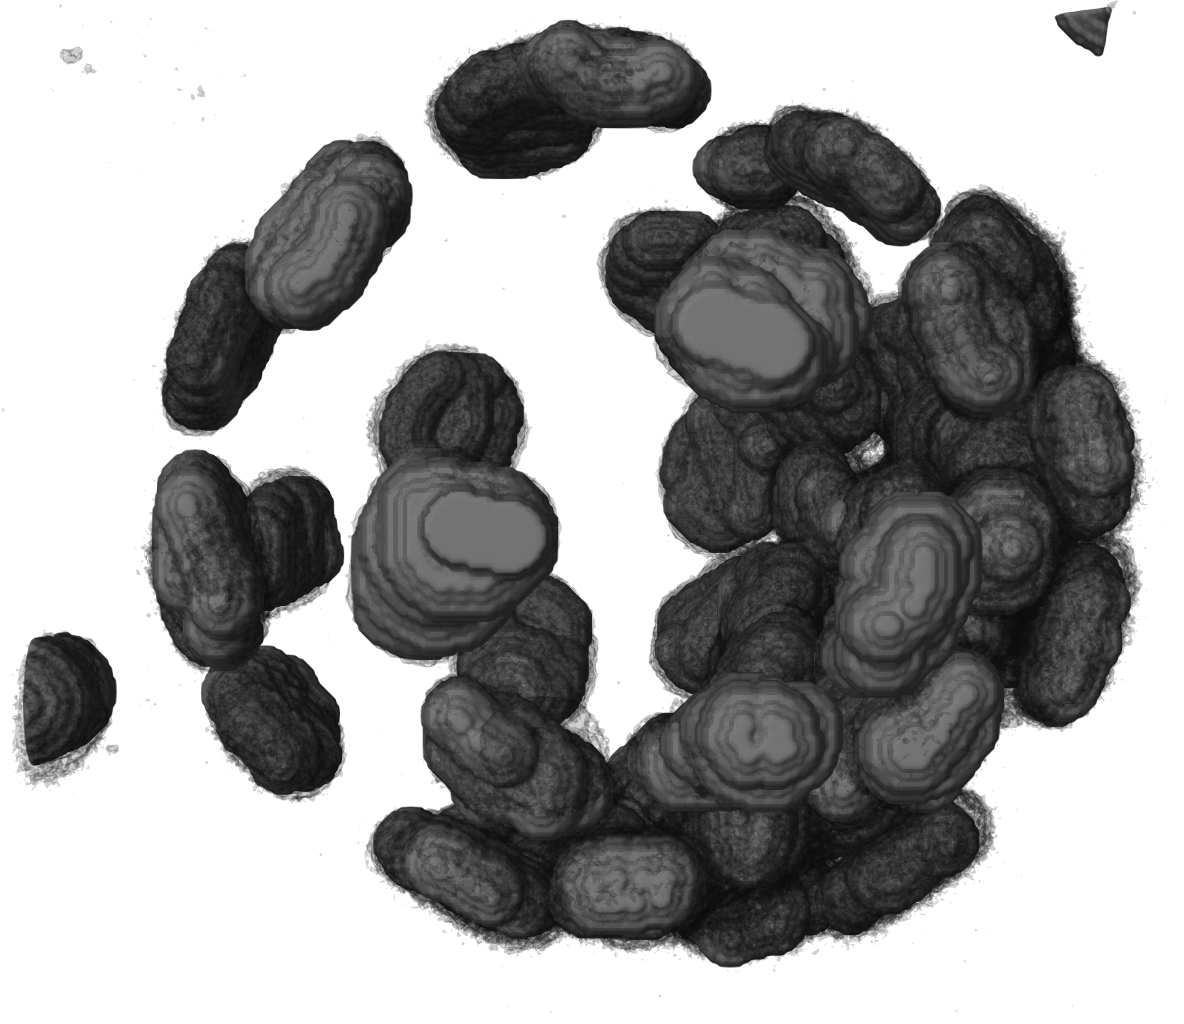
\includegraphics[width=0.4\textwidth]{images/idr-6001240-cvsx.png}}
    \subfigure[MVSX]{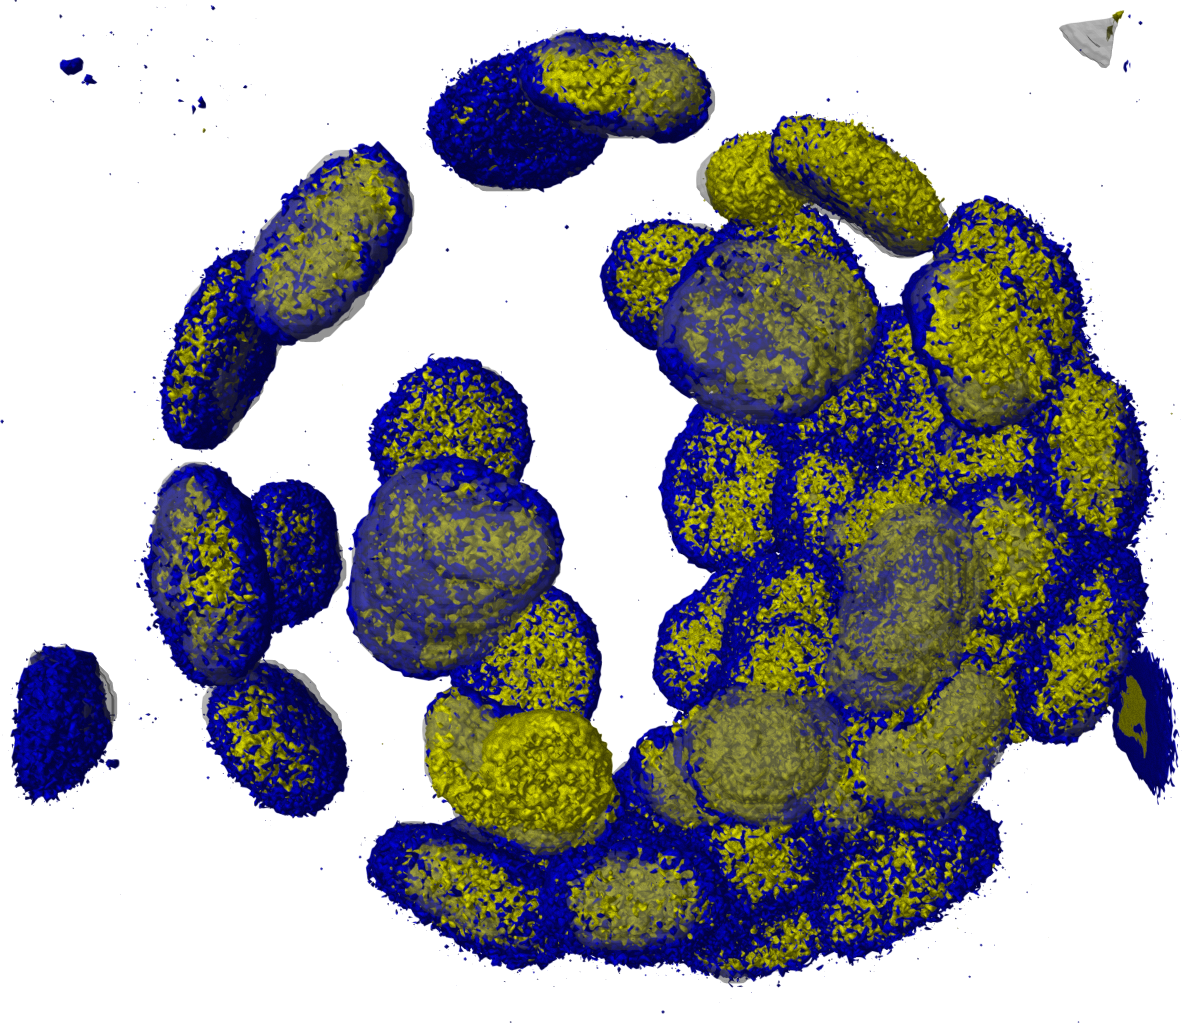
\includegraphics[width=0.4\textwidth]{images/idr-6001240-mvsx.png}}
    \caption[Correction of missing annotations]{Correction of missing color annotations for dataset IDR-6001240.}
  \end{figure}  
\end{frame}

\begin{frame}{Conversion Library --- Improvements}
  \begin{figure}
    \centering
    \subfigure[CVSX]{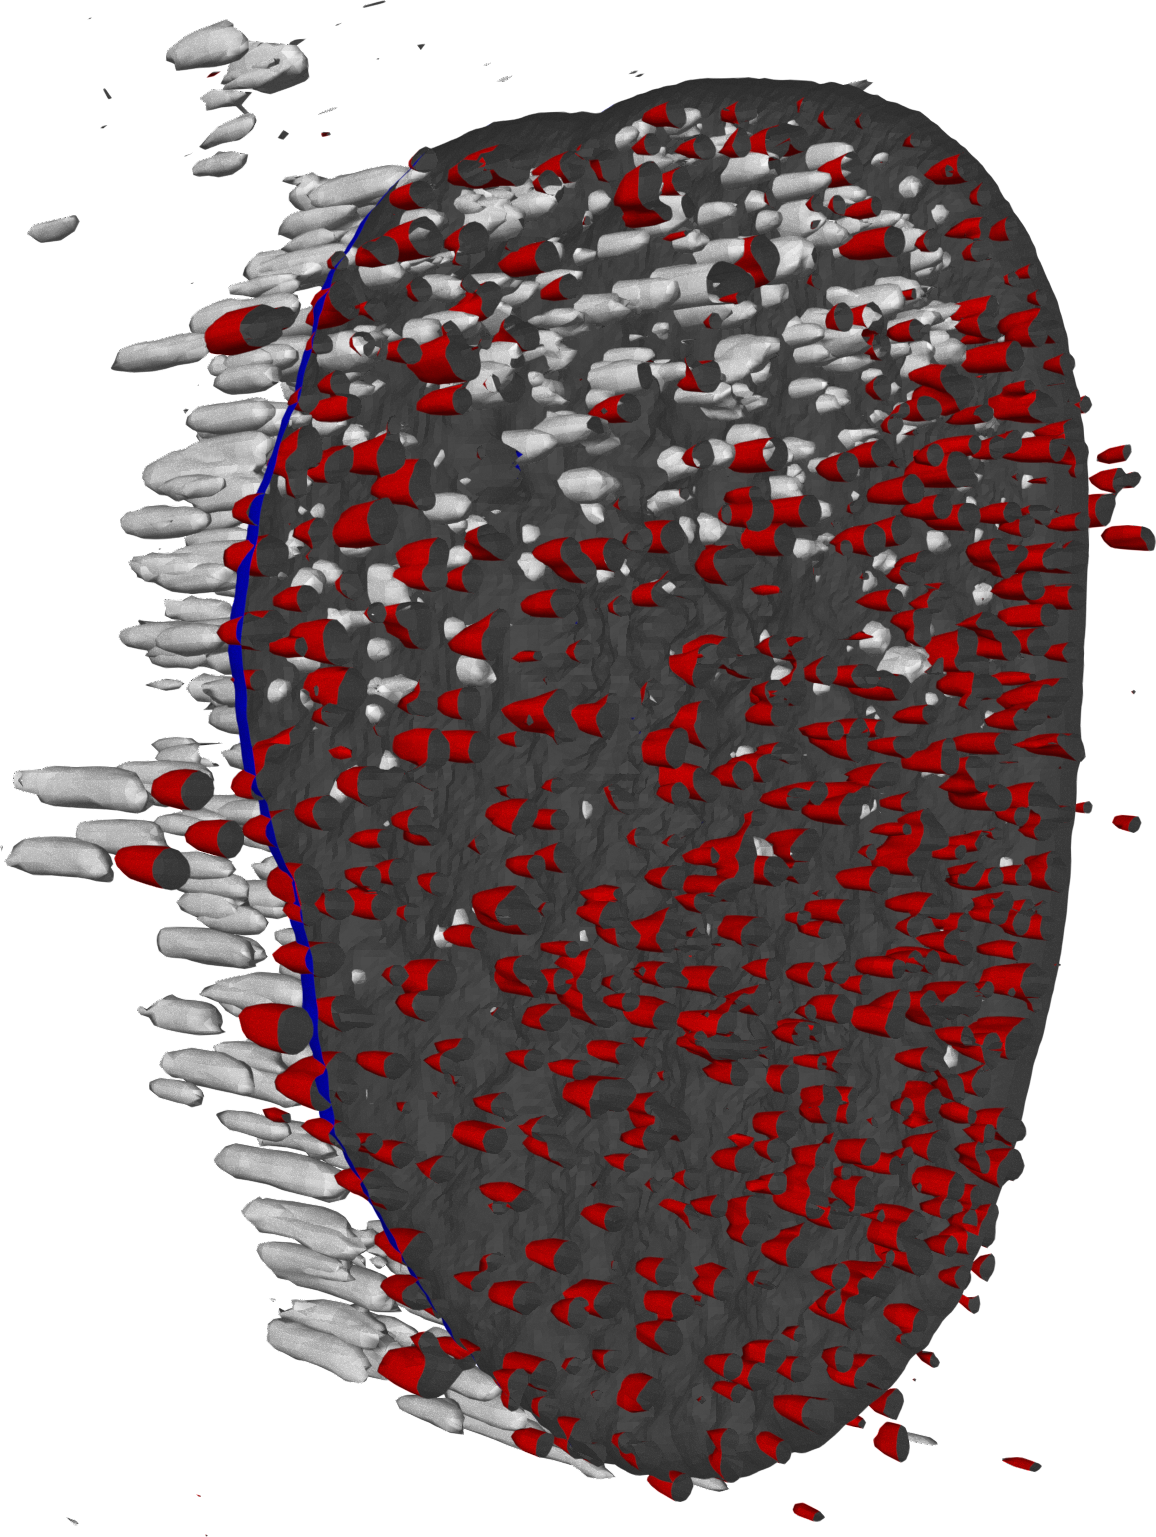
\includegraphics[width=0.3\textwidth]{images/missing-face-cvsx.png}}
    \subfigure[MVSX]{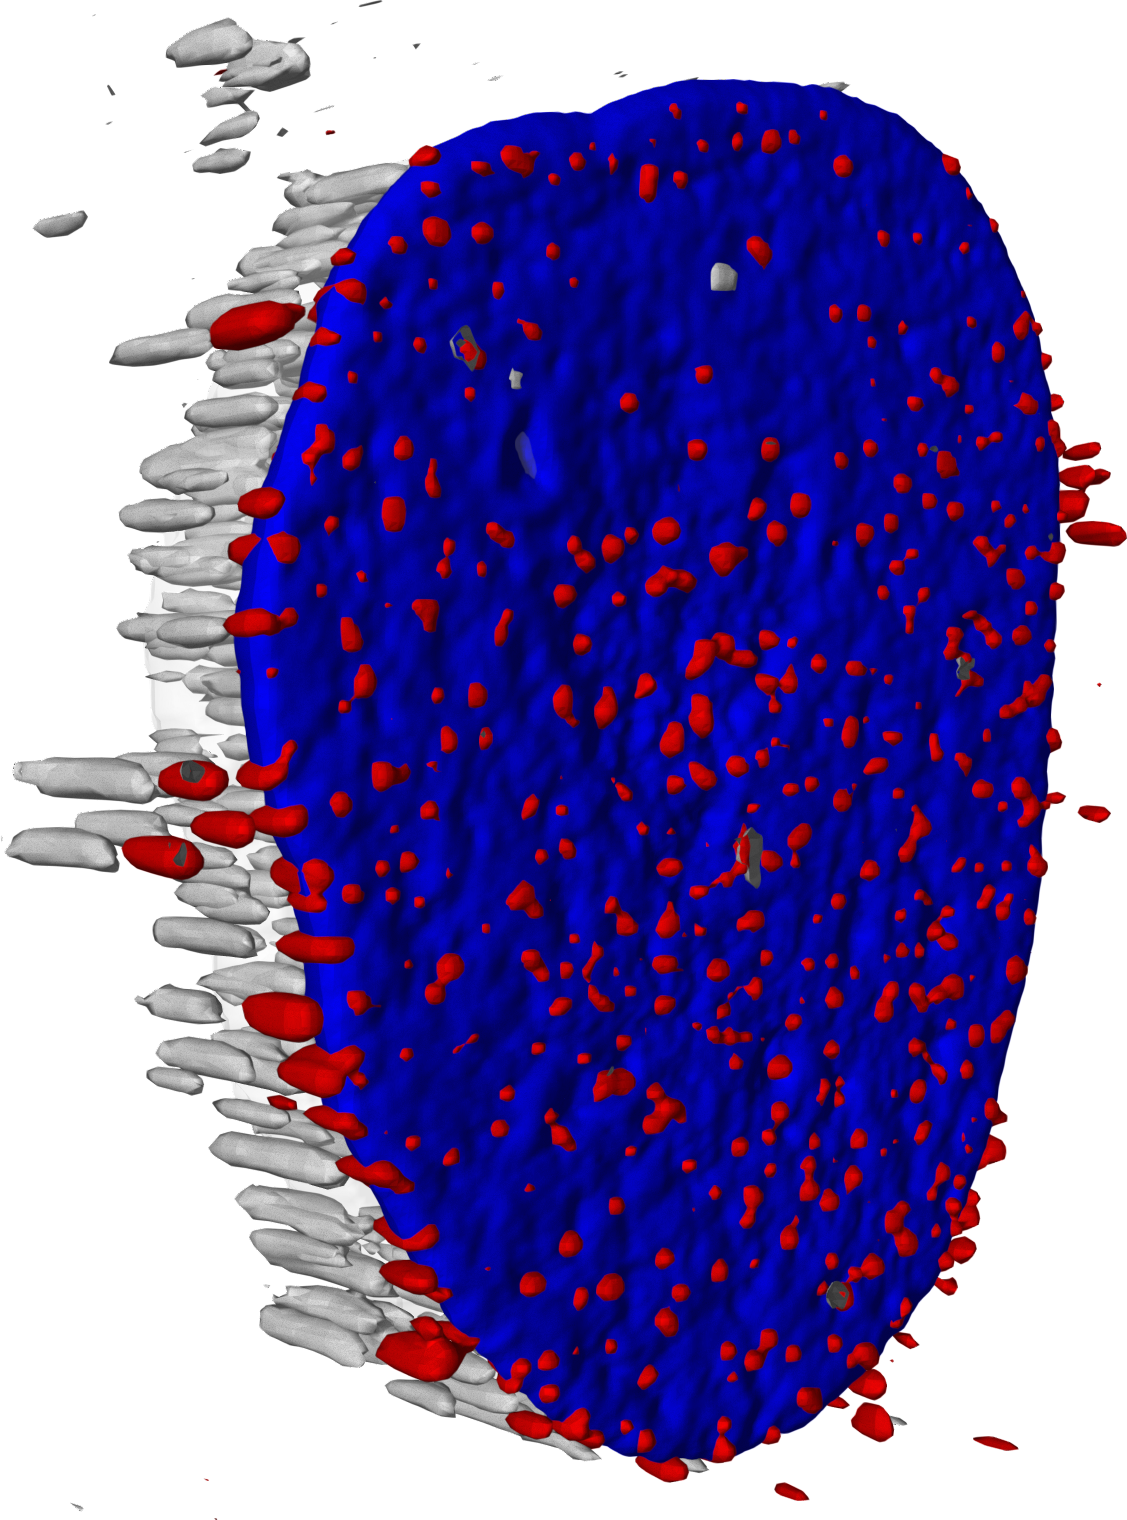
\includegraphics[width=0.3\textwidth]{images/missing-face-mvsx.png}}
    \caption[Correction of isosurface capping]{Correction of isosurface capping for dataset IDR-13457537.}
  \end{figure}  
\end{frame}


\begin{frame}{Web Application}
  \begin{itemize}
    \item The library is a CLI tool; biologists need a GUI
    \item \textbf{Dashboard}: Manage entries and storage quotas
    \item \textbf{WYSIWYG Editor}: Interactively update colors, opacities, and isovalues
    \item \textbf{Sharing}: Persistent URLs and export to MolViewStories
  \end{itemize}
\end{frame}

\begin{frame}{Web Application --- Architecture}
  \textbf{Main Components:}
  \begin{itemize}
    \item \textbf{Frontend:} React SPA
    \item \textbf{Backend:} FastAPI
    \item \textbf{Storage:} PostgreSQL + MinIO
    \item \textbf{Auth:} EINFRA AAI
  \end{itemize}
\end{frame}

\begin{frame}{Web Application --- Deployment}
  \textbf{Infrastructure:}
  \begin{itemize}
    \item Containerized with Docker
    \item Deployed on CERIT-SC Kubernetes cluster
    \item Helm charts for configuration management
    \item CI/CD pipeline via GitHub Actions
  \end{itemize}

  \textbf{Available at:}
  \begin{itemize}
    \item Web: \\ \url{https://web.volseg-editor.dyn.cloud.e-infra.cz/}
    \item API: \\ \url{https://api.volseg-editor.dyn.cloud.e-infra.cz/docs}
  \end{itemize}
\end{frame}

\begin{frame}{Web Application --- Results}
  \begin{figure}
    \includegraphics[width=1\textwidth,height=0.7\textheight,keepaspectratio]{./images/dashboard.png}
    \caption{User's dashboard in the web application.}
  \end{figure}
\end{frame}

\begin{frame}{Web Application --- Results}
  \begin{figure}
    \includegraphics[width=1\textwidth,height=0.7\textheight,keepaspectratio]{./images/preview page.png}
    \caption{Annotations editor the web application.}
  \end{figure}
\end{frame}


\begin{frame}{Conclusion}
  \begin{itemize}
    \item Replaced the Mol* VS client code with declarative MolViewSpec
    \item Corrected rendering artifacts of the legacy client
    \item Democratized access to non-programmers
    \item Simplified getting volume and segmentation data into MolViewStories
    \item Blueprint for the next generation of the Mol* VS preprocessor
  \end{itemize}
\end{frame}

\section{\bibname}
\begin{frame}[t, allowframebreaks, noframenumbering]{\bibname}
\printbibliography[heading=none]
\end{frame}

\begin{frame}[plain,noframenumbering]
Thank You for Your Attention!
\\
\textbf{TODO: add an epic AI generated image}
\end{frame}

\appendix

\section{Otázky oponenta}

\subsection[Otázka 1]{Otázka 1}

\begin{frame}
  \begin{block}{Otázka oponenta 1}
    TODO
  \end{block}
  \begin{itemize}
    \item answer
    \item answer
  \end{itemize}
\end{frame}

\subsection[Otázka 2]{Otázka 2}

\begin{frame}
  \begin{block}{Otázka oponenta 2}
    TODO
  \end{block}
  \begin{itemize}
    \item answer
    \item answer
  \end{itemize}
\end{frame}

\subsection[Otázka 3]{Otázka 3}

\begin{frame}
  \begin{block}{Otázka oponenta 3}
    TODO
  \end{block}
  \begin{itemize}
    \item answer
    \item answer
  \end{itemize}
\end{frame}

\makeoutro
\addtocounter{framenumber}{-1}

\end{document}
